%==============================================================================
% Sjabloon onderzoeksvoorstel bachproef
%==============================================================================
% Gebaseerd op document class `hogent-article'
% zie <https://github.com/HoGentTIN/latex-hogent-article>

% Voor een voorstel in het Engels: voeg de documentclass-optie [english] toe.
% Let op: kan enkel na toestemming van de bachelorproefcoördinator!
\documentclass{hogent-article}

% Invoegen bibliografiebestand
\addbibresource{voorstel.bib}

% Informatie over de opleiding, het vak en soort opdracht
\studyprogramme{Professionele bachelor toegepaste informatica}
\course{Bachelorproef}
\assignmenttype{Onderzoeksvoorstel}
% Voor een voorstel in het Engels, haal de volgende 3 regels uit commentaar
% \studyprogramme{Bachelor of applied information technology}
% \course{Bachelor thesis}
% \assignmenttype{Research proposal}

\academicyear{2023-2024} % TODO: pas het academiejaar aan

% TODO: Werktitel
\title{Ontwikkeling van een Proof-of-Concept Applicatie voor Spraak-naar-tekst Transcriptie van Vlaamse Een-op-een Gesprekken in de Zorgsector}

% TODO: Studentnaam en emailadres invullen
\author{Ayoub AIT CHEIKH AHMED}
\email{ayoub.aitcheikhahmedn@student.hogent.be}

% TODO: Medestudent
% Gaat het om een bachelorproef in samenwerking met een student in een andere
% opleiding? Geef dan de naam en emailadres hier
% \author{Yasmine Alaoui (naam opleiding)}
% \email{yasmine.alaoui@student.hogent.be}

% TODO: Geef de co-promotor op
\supervisor[Co-promotor]{Donald. Vandendriessche (\href{mailto:sigrid.beekman@synalco.be}{donald.vandendriessche@ordina.be})}

% Binnen welke specialisatierichting uit 3TI situeert dit onderzoek zich?
% Kies uit deze lijst:
%
% - Mobile \& Enterprise development
% - AI \& Data Engineering


\specialisation{Mobile \& Enterprise development, AI \& Data Engineering}
\keywords{Spraak-naar-tekstmodelle, TTS, AI, Mobile development }

\begin{document}

\begin{abstract}
Dit onderzoek focust op de evaluatie van spraak-naar-tekstmodellen voor Vlaamse een-op-een gesprekken in de zorgsector, met een nadruk op de verbetering van communicatie met oudere patiënten. De hoofdvraag van het onderzoek is: 'Hoe kunnen spraak-naar-tekstmodellen effectief aangepast worden voor nauwkeurige transcriptie van gesproken Vlaams in de zorgcontext, ter verbetering van de communicatie met oudere patiënten?' Deze vraag wordt ondersteund door deelvragen die zich richten op de technische aanpassing en evaluatie van deze modellen, en op de praktische toepasbaarheid in de zorgcommunicatie.
De methodologie bestaat uit drie fasen: de ontwikkeling van een applicatie met zowel backend- als frontend-componenten, de selectie en evaluatie van spraak-naar-tekstmodellen op basis van snelheid en accuratie, en het verzamelen en analyseren van data uit een-op-eengesprekken. Deze fasen zullen helpen bij het bepalen van de geschiktheid van verschillende modellen voor de specifieke eisen van de Vlaamse zorgcontext.
De verwachte uitkomsten omvatten niet alleen het identificeren van een effectief spraak-naar-tekstmodel, maar ook het ontwikkelen van een proof-of-concept applicatie die een significante verbetering biedt in de communicatie tussen zorgverleners en oudere zorgvragers. Bovendien zal het onderzoek gerichte aanbevelingen leveren voor de implementatie van deze technologie in de zorgpraktijk, gericht op het verbeteren van de interactie en het begrip tussen zorgverleners en oudere patiënten. Het onderzoek beoogt daarmee een waardevolle bijdrage te leveren aan de efficiëntie en kwaliteit van zorgcommunicatie, en benadrukt het belang van technologische innovatie in de persoonsgerichte zorg.
\end{abstract}

\tableofcontents

% De hoofdtekst van het voorstel zit in een apart bestand, zodat het makkelijk
% kan opgenomen worden in de bijlagen van de bachelorproef zelf.
%---------- Inleiding ---------------------------------------------------------

\section{Introductie}%
\label{sec:introductie}

In de hedendaagse zorg- en welzijnssector is er een verschuiving zichtbaar van aanbodgestuurde naar persoonsgerichte zorg. Dit houdt in dat zorgverleners zorg op maat bieden, rekening houdend met de unieke behoeften, voorkeuren, wensen en verwachtingen van elke cliënt of patiënt. Persoonsgerichte zorg vereist dat zorgverleners hun communicatiestijl aanpassen aan de zorgvragers, omdat kwaliteitsvol sociaal contact essentieel is en een positieve invloed heeft op zowel de fysieke als mentale gezondheid en levenskwaliteit van zorgvragers.
Er is echter kritiek op de manier waarop communicatie vaak plaatsvindt tussen zorgverleners en zorgvragers. Deze communicatie wordt soms als ontoereikend en betuttelend beschouwd, waarbij zorgverleners specifiek voor dit onderzoek oudere patiënten, vaak een kinderlijke stijl hanteren, gekenmerkt door een overdreven toonhoogte, eenvoudige taal en het gebruik van verkleinwoorden en troetelnamen, een stijl die bekend staat als 'secondary babytalk'.

In 2023 vertoont de bevolkingspiramide van het Vlaamse Gewest het kenmerkende profiel van een vergrijzende bevolking, met een toenemend percentage van 65-plussers (21\%) ten opzichte van 2000 (17\%). Dit demografische verandering brengt nieuwe uitdagingen met zich mee in de zorgsector, met name wat betreft de communicatie tussen zorgverleners en zorgbehoevenden in deze leeftijdscategorie.

De vergrijzing van de bevolking leidt tot een toename in het aantal ouderen die zorg nodig hebben, vaak met specifieke communicatiebehoeften. Dit kan variëren van gehoorproblemen tot cognitieve uitdagingen. Hierin ligt het belang dit mijn onderzoek: Een applicatie ontwikkelen die kenmerken van ‘secondary babytalk’ kan identificeren aan de hand van bepaalde speech-to-text modellen die beschikbaar zijn op de markt. Deze modellen zullen met elkaar vergeleken worden aan de hand van specifieke criteria. Dit zal resulteren dat het meest accurate model verkozen kan worden
\textcite{Vlaanderen.be}.

%---------- Stand van zaken ---------------------------------------------------

\section{State-of-the-art}%
\label{sec:state-of-the-art}
\subsection{Probleemstelling}
\begin{quote}
   `` Hoe kunnen we spraak-naar-tekstmodellen evalueren om te bepalen welk model optimaal presteert voor de specifieke usecase van spraaktranscriptie, met als doel het identificeren en verminderen van 'secondary babytalk' in een-op-een gesprekken tussen zorgverleners en oudere zorgvragers binnen de Vlaamse zorgsector, streven naar een respectvolle en doeltreffende communicatie te bevorderen?''

\end{quote}

Om deze onderzoeksvraag te kunnen beantwoorden, is een systematische aanpak vereist.

Daarvoor moet een literatuurstudie worden uitgevoerd. In deze context dienen begrippen gedefinieerd te worden. Allereerst moet beschreven worden wat een speech-to-text model precies inhoudt en waar het zich bevindt in de wereld van kunstmatige intelligentie. Welke modellen zijn beschikbaar op de markt? En wat zijn de criteria om deze modellen te testen?

\subsection{Spraak-naar-tekst}

Het begrijpen van de nuances tussen termen zoals spraakherkenning, stemherkenning en natuurlijke taalverwerking kan uitdagend zijn. In de loop van mijn onderzoek heb ik een mogelijke verduidelijking geïdentificeerd voor deze conceptuele complexiteit.

\autocite{IBM} defineert het als volgt: \\Spraakherkenning, ook wel bekend als automatische spraakherkenning (ASR), computergestuurde spraakherkenning of spraak-naar-tekst, is een functie die een programma in staat stelt menselijke spraak te verwerken en om te zetten in geschreven tekst. Hoewel het vaak verward wordt met stemherkenning, richt spraakherkenning zich op de vertaling van spraak van een verbale vorm naar een tekstuele, terwijl stemherkenning alleen probeert de stem van een individuele gebruiker te identificeren.

Spraakherkenningsmodellen produceren een transcript van spraak in audiogegevens. Dit transcript kan op zichzelf worden gebruikt of verder worden verwerkt voor andere doeleinden, zoals het gebruik van grote taalmodellen om de inhoud van de spraak te analyseren \autocite{OConnor2023}.

Samengevat Spraakherkenning, ook bekend als automatische spraakherkenning (ASR), is de mogelijkheid van een programma om gesproken taal om te zetten naar geschreven tekst.

\subsection{Beschikbaar modellen}
\subsubsection{Google Speech to Text}

Google Cloud Speech-to-Text is een API van Google Cloud Platform die gesproken taal omzet in geschreven tekst. Het ondersteunt verschillende talen, real-time streaming en batchverwerking. Gebruikers kunnen de service aanpassen voor domeinspecifieke termen en het integreert naadloos met andere Google Cloud-services. De API biedt veilige en nauwkeurige spraakherkenning voor verschillende toepassingen.\autocite{DocsGoogle}
\subsubsection{AssemblyAI}
Samengesteld door AI-experts, omvatten de spraak-AI-modellen van AssemblyAI nauwkeurige spraak-naar-tekst voor spraakgegevens (zoals gesprekken, virtuele vergaderingen en podcasts), sprekerdetectie, sentimentanalyse, hoofdstukdetectie, PII-verwijdering en meer \autocite{DocsAssemblyai}.
\subsection{Criteria}
%----------TODO THIS NEED TO BE REVIEWED 
Uiteindelijk komt een juiste evaluatie neer op het aannemen van een wetenschappelijke benadering om ervoor te zorgen dat de resultaten accuraat, herhaalbaar en betrouwbaar zijn. Laten we nu onderzoeken hoe kunnen de gekozen modellen getest worden.

\subsubsection{Word Error Rate (WER)}
Automatische spraakherkenningssystemen (ASR) hebben de afgelopen tien jaar aanzienlijke vooruitgang geboekt, waarbij de Word Error Rate (WER) naar voren is gekomen als de voornaamste maatstaf voor het evalueren van de prestaties van deze systemen. WER is gebaseerd op het concept van de bewerkingsafstand en kwantificeert de nauwkeurigheid van ASR door de verhouding van invoegingen, verwijderingen en vervangingen ten opzichte van het totale aantal tokens in een zin te berekenen. Deze maatstaf is bijzonder effectief voor talen zoals het Engels, die doorgaans één spelling voor elk woord hebben, waardoor WER de algehele correctheid nauwkeurig kan weerspiegelen door de getranscribeerde tekst te vergelijken met de oorspronkelijke spraak.\\
\autocite{Raghavan2022}.
\\De \(WER\) kan berekend worden als volgt:

\begin{equation}
   WER(w) = \frac{i + d + s}{N_t}
\end{equation}
waarbij:
\begin{itemize}
    \item \(i\) is het aantal invoegingen
    \item \(d\) is het aantal verwijderingen
    \item \(s\) is het aantal substituties
    \item \(N\) is de totale aantal woorden
\end{itemize}

In het bijzonder telt WER inserties, waarbij het model een woord transcribeert dat niet aanwezig is, verwijderingen, waarbij het model een woord dat aanwezig is niet transcribeert en substituties, waarbij het model een woord onjuist transcribeert
\autocite{OConnor2023}.
\begin{figure}[htbp]
    \centering
    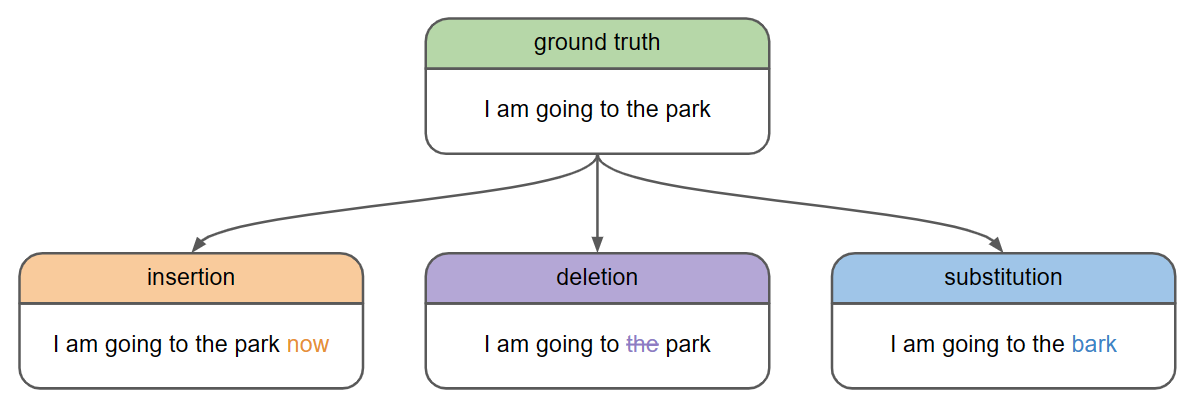
\includegraphics[width=0.5\textwidth]{wer_1}
    \caption{Een referentietranscript samen met één voorbeeld van elk van de 3 soorten fouten die WER telt \autocite{OConnor2023}.}
    \label{fig:WER count}
\end{figure}

WER wordt beïnvloed door verschillende factoren, waaronder technische taal, branchespecifieke termen, accenten en ruis in de audiogegevens. Het herkennen van technische en gespecialiseerde taal vereist extra inspanning, terwijl accenten en diverse audiogegevens mogelijk aangepaste modellen nodig hebben voor nauwkeurige transcriptie. De aanwezigheid van ruis, veelvoorkomend in real-world scenario's zoals telefoongesprekken en diverse omgevingen, vormt een uitdaging voor de nauwkeurigheid van spraakherkenningssystemen \autocite{Gevirtz2018}.

Echter zou WER alleen voldoende zijn als criterium omdat het fouten berekent op hetzelfde niveau, maar omdat het wat vaak niet het geval is moeten we een andere metriek introduceren \autocite{OConnor2023}.
\subsubsection{Jaro–Winkler distance (JW)}


De Jaro-Winkler Distance is een algoritme voor het meten van de gelijkenis tussen twee teksten en wordt voornamelijk gebruikt op het gebied van duplicatiedetectie. Dit algoritme is gebaseerd op het Jaro-Distance algoritme, dat is ontwikkeld door Matthew A. Jaro en later verder ontwikkeld door William E. Winkler en Thibaudeau door de Jaro Distance aan te passen om hogere gewichten te geven aan overeenkomsten in de voorvoegsels. Hoe hoger de waarde van de Jaro-Winkler Distance voor twee teksten is, hoe groter de gelijkenis tussen beide teksten. Een normale waarde van 0 duidt op geen gelijkenis, en een waarde van 1 duidt op de aanwezigheid van exacte overeenkomsten. De Jaro-Winkler-Distance formule wordt gebruikt om de afstand (dj) tussen de twee teksten  S1 en S2 te berekenen \autocite{Brinardi2017}.

De \(JW\) tussen twee strings kan berekend worden als volgt:

\[
JW = \frac{1}{3} \left( \frac{m}{\text{{length}}(s1)} + \frac{m}{\text{{length}}(s2)} + \frac{m - t}{m} \right)
\]

waarbij:
\begin{itemize}
    \item \(m\) is het aantal overeenkomende karakters
    \item \(t\) is het aantal transposities
\end{itemize}
Anders gezegd Jaro-Winkler similarity is de maatstaf voor gelijkenis tussen twee teksten. De waarde van de Jaro-afstand varieert van 0 tot 1, waarbij 1 betekent dat de teksten identiek zijn en 0 betekent dat er geen gelijkenis is tussen de twee teksten.

% Voor literatuurverwijzingen zijn er twee belangrijke commando's:
% \autocite{KEY} => (Auteur, jaartal) Gebruik dit als de naam van de auteur
%   geen onderdeel is van de zin.
% \textcite{KEY} => Auteur (jaartal)  Gebruik dit als de auteursnaam wel een
%   functie heeft in de zin (bv. ``Uit onderzoek door Doll & Hill (1954) bleek
%   ...'')

%---------- Methodologie ------------------------------------------------------
\section{Methodologie}%
\label{sec:methodologie}
Dit onderzoek richt zich op het evalueren van diverse speech-to-textmodellen om kenmerken van secondary babytalk te identificeren in gesprekken tussen zorgvragers en studentzorgverleners. De methodologie is opgedeeld in drie hoofdfasen:
\subsection{Fase 1: Applicatie opbouwen \\ (November 2023 - Februari 2024)}
subsubsection{Backend}
De backend van de applicatie heeft de verantwoordelijkheid om een invoer te verwerken, wat in dit geval een geluidsopname van het gesprek is.

Vervolgens maakt het een API-oproep naar verschillende speech-to-textmodellen, afhankelijk van welk model de gebruiker heeft geselecteerd. Na het verkrijgen van de respons van het gekozen model, stuurt de backend deze respons door naar de frontend, waar deze verder wordt verwerkt.

In essentie fungeert de backend als een tussenliggende component die de communicatie tussen de frontend en de verschillende speech-to-textmodellen mogelijk maakt.

Het is echter van belang om Python te erkennen als een zeer aanbevolen programmeertaal voor AI-projecten. Deze keuze sluit aan bij het inzichtelijke perspectief van Damian hill:

Python is uitgegroeid tot een veelzijdige programmeertaal voor kunstmatige intelligentie en datawetenschap, dankzij zijn eenvoud, grote gemeenschap, uitgebreide bibliotheken en naadloze integratiemogelijkheden. De leesbaarheid en robuustheid maken het een ideale keuze voor zowel beginners als ervaren ontwikkelaars. Met het voortdurend groeiende ecosysteem van Python is er geen twijfel dat het een cruciale rol zal blijven spelen in het veld van kunstmatige intelligentie en datawetenschap. \autocite{Hill2023}.

Nochtans is de optimale programmeertaal voor backend-ontwikkeling, rekening houdend met mijn achtergrond en mijn streven naar verdere vaardigheidsontwikkeling, omvat het gebruik van Java in combinatie met Spring Boot. Gezien mijn aanzienlijke ervaring met Java, is deze keuze bijzonder voordelig. Bovendien biedt deze voorkeur potentiële voordelen voor studenten en onderzoekers die zich voor het eerst bezighouden met Java-programmering, met name in het kader van hun initiële betrokkenheid bij Speech to text Recognition.

\subsubsection{Frontend}
De front-end in deze context kan uiteindelijk een Android-toepassing zijn om de respons van de backend weer te geven. Dit kan verschillende voordelen hebben ten opzichte van een webtoepassing, zoals die in de vorige onderzoek.\\
\textbf{Offlinefunctionaliteit}:

Een Android-app kan ontworpen worden om offline te werken, waardoor het elderspeak-detectie kan blijven monitoren, zelfs wanneer het apparaat niet is verbonden met internet. Dit is vooral handig in scenario's waar een stabiele internetverbinding niet is gegarandeerd.\\
\textbf{Gebruiksvriendelijk:}

Een Android-app kan zeer handig zijn bij het werken in de gezondheidszorgsector.

De smartphone kan naar een bepaalde locatie worden meegenomen en vervolgens gebruikt worden om de app-functionaliteit te gebruiken in plaats van te gedwongen worden een desktopcomputer te gebruiken. Bovendien kan de gebruiker een interactieve ervaring krijgen, bijvoorbeeld door meldingen te ontvangen over een proces of functionaliteit.
\subsection{Fase 2: Evaluatie en Selectie van Modellen \\ (Februari 2024 - Maart 2024)}
In deze fase van het onderzoek wordt een reeks specifieke stappen ondernomen om de geschiktheid van verschillende speech-to-textmodellen te beoordelen en uiteindelijk het meest geschikte model te selecteren voor verdere analyse.
\subsubsection{Implementatie van Modellen in de Backend:}
De geselecteerde speech-to-textmodellen worden geïntegreerd in de backend van de applicatie. Deze implementatie omvat het configureren van de modellen om te communiceren met de applicatie-infrastructuur en het mogelijk maken van verzoeken vanuit de frontend.

\subsubsection{Evaluatie van Modellen:}
De geïmplementeerde modellen worden onderworpen aan een grondige evaluatie op verschillende metrieken zoals in de vorige sectie vermeld wordt.
Deze fase is cruciaal omdat het de basis legt voor het gebruik van een specifiek speech-to-textmodel binnen de applicatie.

\subsection{Fase 3: Dataverzameling en \\ Analyse \\ (Maart 2024 - April 2024)}
Het verzamelen van één-op-één-gesprekken tussen Vlaams-sprekende zorgvragers en student-zorgverleners staat centraal in deze fase. Hierbij streven we naar een zorgvuldige samenstelling van een representatieve dataset die een breed reeks aan contexten binnen de zorgsector bedekt.

In de volgende stap zullen we de geselecteerde speech-to-textmodellen evalueren en testen. Dit omvat de conversie van audiogesprekken naar tekst met behulp van het gekozen spraak-naar-tekstmodel. Om de kwaliteit van de transcripties te waarborgen, zal er ook een handmatige validatie plaatsvinden, uitgevoerd door een medestudent. Verdere details hierover ontvang je later. Deze evaluatie en testfase is cruciaal voor het begrijpen van de prestaties en toepasbaarheid van het gekozen model in de context van ons onderzoek.\\
De samenvatting van bevindingen biedt een overzicht van de prestaties en karakteristieken van de onderzochte modellen, terwijl de vergelijking een diepgaande analyse geeft van hun sterke punten en beperkingen. De resulterende aanbevelingen zullen dienen als leidraad voor de keuze van het optimaal spraak-naar-tekstmodel dat het meest geschikt is voor de specifieke vereisten van de secondary babytalk-toepassing. Hierdoor streven we naar een effectieve implementatie van spraaktechnologie om de communicatie tussen zorgvragers en student-zorgverleners te verbeteren.
%---------- Verwachte resultaten ----------------------------------------------
\section{Verwacht resultaat, conclusie}%
\label{sec:verwachte_resultaten}
In deze sectie van mijn onderzoek, na de uitvoering van de methodologie en testen, verwacht ik dat de resultaten zullen aantonen dat het geselecteerde speech-to-textmodel succesvol is in het identificeren van kenmerken van secondary babytalk in 1-op-1-gesprekken tussen Vlaams-sprekende zorgvragers en student-zorgverleners. De geplande grafieken en metingen zullen waarschijnlijk de nauwkeurigheid van het model illustreren, vooral in diverse contexten binnen de zorgsector. Op basis van deze verwachte resultaten concludeer ik mogelijk dat het gekozen model een waardevolle bijdrage kan leveren aan het verbeteren van de communicatie tussen zorgvragers en student-zorgverleners. Dit zou resulteren in aanbevelingen voor de integratie van dit specifieke model in de secondary babytalk-applicatie, waardoor een verhoogde effectiviteit en relevantie worden bereikt in de context van de gezondheidszorg.



\printbibliography[heading=bibintoc]

\end{document}